% WP X: "WP name"
% Deliverable DX.Y: "Name of this deliverable"
%
% Editors: Name and Surname of the Editor
% List of Authors:
%

\documentclass{SmartReport}
\usepackage{url, rotating}

\usepackage{subfig}
\usepackage{color}
\usepackage{paralist}
\usepackage{tabularx}
\usepackage{arydshln}
\usepackage{longtable}
\usepackage{tabu}
\usepackage{booktabs}

\definecolor{ao(english)}{rgb}{0.0, 0.5, 0.0}

\newcommand{\todo}[1]{\noindent{\textcolor{red}{[TODO: #1]}}}

\begin{document}
\wpnumber{4} \wptitle{Peer Modeling and Search}
\instshort{UH} \delnumber{4.3} \versionnumber{0.1}
\contribshort{UH}
\deltitle{First Version of the Peer Search in Smart Societies}
\delshorttitle{Peer Search} 
\delavail{PU}
\delstatus{RD}	
\duedate{30/6/2014}
\deldate{\today}
\delowner{Daniele Miorandi}
\wpleader{Alethia Hume, UNITN}
\qualityassessor{Hong-Linh Truong}
\smartkeywords{peer manager, search, privacy, ranking}
\maketitle

\begin{smartcontributors}
%date & reviewer (individual)\\
%0.1 & 04/11/2014 & 
UH & Daniele Miorandi \\
UNITN & Alethia Hume, Ronald Chenu\\
\end{smartcontributors}

%define the abstract
\begin{smartabstract}
%\textcolor{red}{Executive summary: max 1 page, objectives of the deliverable, achievements and impact on the project as a whole.}

This deliverable reports the outcomes of the activities carried out in WP4 on the peer profiling schemas and the privacy-aware mechanisms defined for the Peer Manager (PM). In particular, it includes a detailed description of the implementation and integration into the project infrastructure as well as the definition of evaluation procedures. 
%The main focus of the reporting period was the identification of appropriate evaluation mechanisms and the definition of an evaluation plan that should be inline also with the overall project evaluation.
Another achievement described in the deliverable  %during this period of the Smart Society project 
is the definition and initial integration of the privacy-enhancing component of the PM (integration with PrimeLife Policy Language), which is a fundamental building block for managing the information of peers in a privacy-preserving manner. 

Content-wise, the deliverable presents:
%\begin{enumerate}
\begin{inparaenum}[\itshape (i)]
\item The mechanisms and implementation details for the profile schemas and the privacy-enhancing technologies used by the PM;
\item The mechanisms and implementation details for the services that allow searching, matching and ranking of peers based on different attributes (i.e., characteristics) from their profiles;
\item The evaluation plans for WP4 including analytical and user-based evaluations; and
\item The description of how the PM is currently integrated in the SmartSociety platform and used in different project-wide scenarios.
\end{inparaenum}
%\end{enumerate}

%It is important to note also that while an evaluation plan is presented in this document, the actual evaluation and therefore the implementation of such plan will start during the second half of year 3 and will be formally reported as part of deliverable D4.4.
\end{smartabstract}


\section*{List of Acronyms}
\begin{tabular}{|c|p{3cm}|p{10cm}|}
\hline 
\textbf{Acronym} & \textbf{Full Name} & \textbf{Description} \\
\hline 
\hline 
%EC & Evaluator Component & System component in charge of evaluating the outcomes of each computation task (Sec.~\ref{sec:evaluator}).\\
%\hline 
CM & Context Manager & System componet in charge of monitoring the
context the agent represented on the platform by a peer is in.\\
\hline
HDA-CAS & Hybrid and Diversity-Aware Collective Adaptive Systems & The
type of systems focus of the SmartSociety project, characterized by
hybrid (people and machines) collectives able to work seamlessly
together through the awareness of diversity. \\ 
\hline
IM & Incentives Manager & System component in charge of managing the implementation of incentive schemes.\\  
\hline 
KB & Knowledge Base &  System component in charge of storing and managing the knowledge in the platform.\\
\hline
OM & Orchestration Manager &  System component in charge of
orchestrating the lifecycle of tasks on the SmartSociety platform. \\
\hline 
PF & Programming Framework &  System component in charge of exposing
appropriate primitives and interfaces to application developers.\\
PPL & PrimeLife Policy Language & A generic language for expressing
privacy policies, developed within the scope of the PrimeLife
EC-funded project. \\
\hline 
PM & Peer Manager &  System component in charge of managing peers.\\
\hline \\
PS & Provenance Store & System component in charge of logging actions performed by platform components and peers.\\
\hline
RM & Reputation Manager & System componet in charge of handling the reputation of any system resource, including peers. \\
\hline
SmartCom & Communication Middleware & System component in charge of managing
communication channels between the platform and the peers. \\
\hline
\end{tabular}

\newpage

%%%%%%%%%%%%%%%%%%%%%%%%%%%%%%%%%%%%%%%%%%%%%%%%%%%%%%%%%%%%%%%%%%%%%%%%%%%%%%%%%%%%%%%%%%%%%%%%%%%%%%%%%%%%%%%%%%%%%%%%
%%%%%%%%%%%%%%%%%%%%%%%%%%%%%%%%%%%%%%%%

\section{Introduction}
\label{sec:intro}
This deliverable reports the work done on tasks T4.3 and T4.4. In particular, T4.3 covers the description of profiling mechanisms and privacy-aware algorithms including those for searching and ranking of peers. On the other hand, T4.4 refers to the implementation and integration of these mechanisms into the project infrastructure as well as the definition of an plan for evaluating them.

During the second year of the project, the WP4 worked on the refinement of models for data and knowledge representation and for privacy-aware storage, as well as the definition of mechanisms for matching atomic-tasks with peers and ranking matching results. 
As such, the main outcome was the definition of the \emph{Peer Manager (PM)} component as a privacy-aware storage for the information of peers in the SmartSociety platform. This definition included also the specification of a privacy-by-design architecture for the PM. The results of this work were reported in deliverable D4.2.
Although the focus of year 2 was on the definition of models and mechanisms, an initial prototype of the PM was also developed during such period and the early reports of this implementation was included in the deliverable D4.2.


The main objectives of this year (year 3 of the SmartSociety project) are:
\begin{enumerate}
\item Provide a more complete implementation and integration of models and mechanisms proposed during the year 2 of the project.
\item The application of evaluation procedures that include the definition of an evaluation plan and its subsequent implementation.
\end{enumerate}
In this regard, it is important to note that this deliverable covers only partially the work towards the above mentioned objectives (i.e., until M30). As a consequence, only the definition of a plan for evaluation is presented in this document while its execution is planned for the second half of year 3 and the report of the evaluation results will be presented in the next deliverable.

The reminder of the deliverable is organized as follows, \ldots 

%%%%%%%%%%%%%%%%%%%%%%%%%%%%%%%%%%%%%%%%
%%%%%%%%%%%%%%%%%%%%%%%%%%%%%%%%%%%%%%%%%%%%%%%%%%%%%%%%%%%%%%%%%%%%%%%%%%%%%%%%%%%%%%%%%%%%%%%%%%%%%%%%%%%%%%%%%%%%%%%%
\newpage


%%%%%%%%%%%%%%%%%%%%%%%%%%%%%%%%%%%%%%%%%%%%%%%%%%%%%%%%%%%%%%
%\section{Profiling}
\section{Profile Schemas and Privacy-aware Mechanisms}
\label{sec:profiling}
%\todo{RONALD - first draft by 30/May}

The \emph{Peer Manager (PM)} is a fundamental building block of the SmartSociety platform, providing a peer-centered data store that maintains and manages information about human- or machine-based peers within a privacy-preserving framework. 

\subsection{Mechanisms and algorithms}
%\todo{Peer Manager Theory - including flow diagram, pseudo-code if needed, whatever explain how it works}

The PM was designed as an extension of existing identity management systems, with the objective of keeping the information owned by peers private.
In order to provide a flexible management of information, the PM builds upon the notion of an \emph{entity-centric semantic enhanced model} that defines an extensible set of entity schemas providing the templates for an attribute-based representation of peers' characteristics~\cite{Giunchiglia_fromknowledge}. Additionally, the PM defines a \emph{storage and privacy protection model} by adding privacy regulations and considerations~\cite{Hartswood:2015fe}. 
The design of this model pays special attention to different privacy issues discussed by the Council of Europe in its recommendation {\sc{cm}}/{\sc{rec}}(2010)13 on profiling \cite{CoE2010}, as well as 
basic legal privacy principles enacted by the {\sc{eu}} Data Protection Directive 95/46/{\sc{ec}} \cite{EUDir95} and that affects profiles when they involve the storage and processing of personal data.

An important feature of the SmartSociety PM model is that the concrete meaning of schemas is further specified by mapping single elements (i.e., types of entities, the names of attributes and their values) to concepts from an underlying ontology that is also part of the same model~\cite{Giunchiglia_fromknowledge}. This design provides additional flexibility in the operations supported, allowing reasoning over peer's properties as well as the implementation of semantic-enhanced services.
%
The basic set of schemas/templates can be easily extended to support new application-specific scenarios requiring, for instance, the creation of new types of peers. The adaptability is provided by enabling the search and information sharing services to work over the new types in a way that is transparent to the rest of the HDA-CAS platform.

%%% Privacy%%%
A key feature of the PM is that the privacy of peers is protected by allowing people (i.e. users) to define profiles that contain and reveal only partial or (semantically) obfuscated information that is used for replying to information requests from other modules/components and is thus enforcing data minimisation. 
This allows, for example, a human peer to reveal whether it is a smoker and its age range (as a way to obfuscate the age and date of birth) when participating in a ride-sharing collective, while the same information can be hidden (i.e., completely obfuscated) when participating in a question-answering collective.

%%% Architecture %%%
The details about the internal architecture of the PM was presented in~\cite{D4.2,Hartswood:2015fe}, however, we recall one of its main component (i.e., the Peer Base) in the conceptual view shown in Figure~\ref{fig:peerManagerPlatform}. The Peer Base is composed of the following sub-components: 
\begin{itemize}
\item A \emph{Platform-Wide Knowledge Base} (${KB}_{PW}$) that stores the core entity types and the underlying ontology, allowing interoperability among SmartSociety components. 
\item A \emph{Platform-Wide Entity Base} (${EB}_{PW}$) that stores entity instances of general interests as well as public profiles of peers (i.e., information that each peer decides to publish in the platform about themselves).
\item A \emph{Knowledge Base} (${KB}_i$) and an \emph{Entity Base} (${EB}_i$) for each peer, which store the peer’s information. The peer maintains control over its data space and defines the privacy policies that apply to the data stored in it. 
%The peer's $KB$ is bootstrapped with the content of the platform-wide's $KB$, which then can be extended/specialized by the peer. The peer's $EB$ stores entity instances that are relevant to the peer (i.e., peer’s personal information, its resources, locations, roles, tasks, etc.). 
\end{itemize}
This storage separation for each of the peers and the platform is one of the Privacy-by-Design decisions taken by WP4 in accordance to the PM  privacy protection model.
%

\begin{figure}[t]
	\centering
	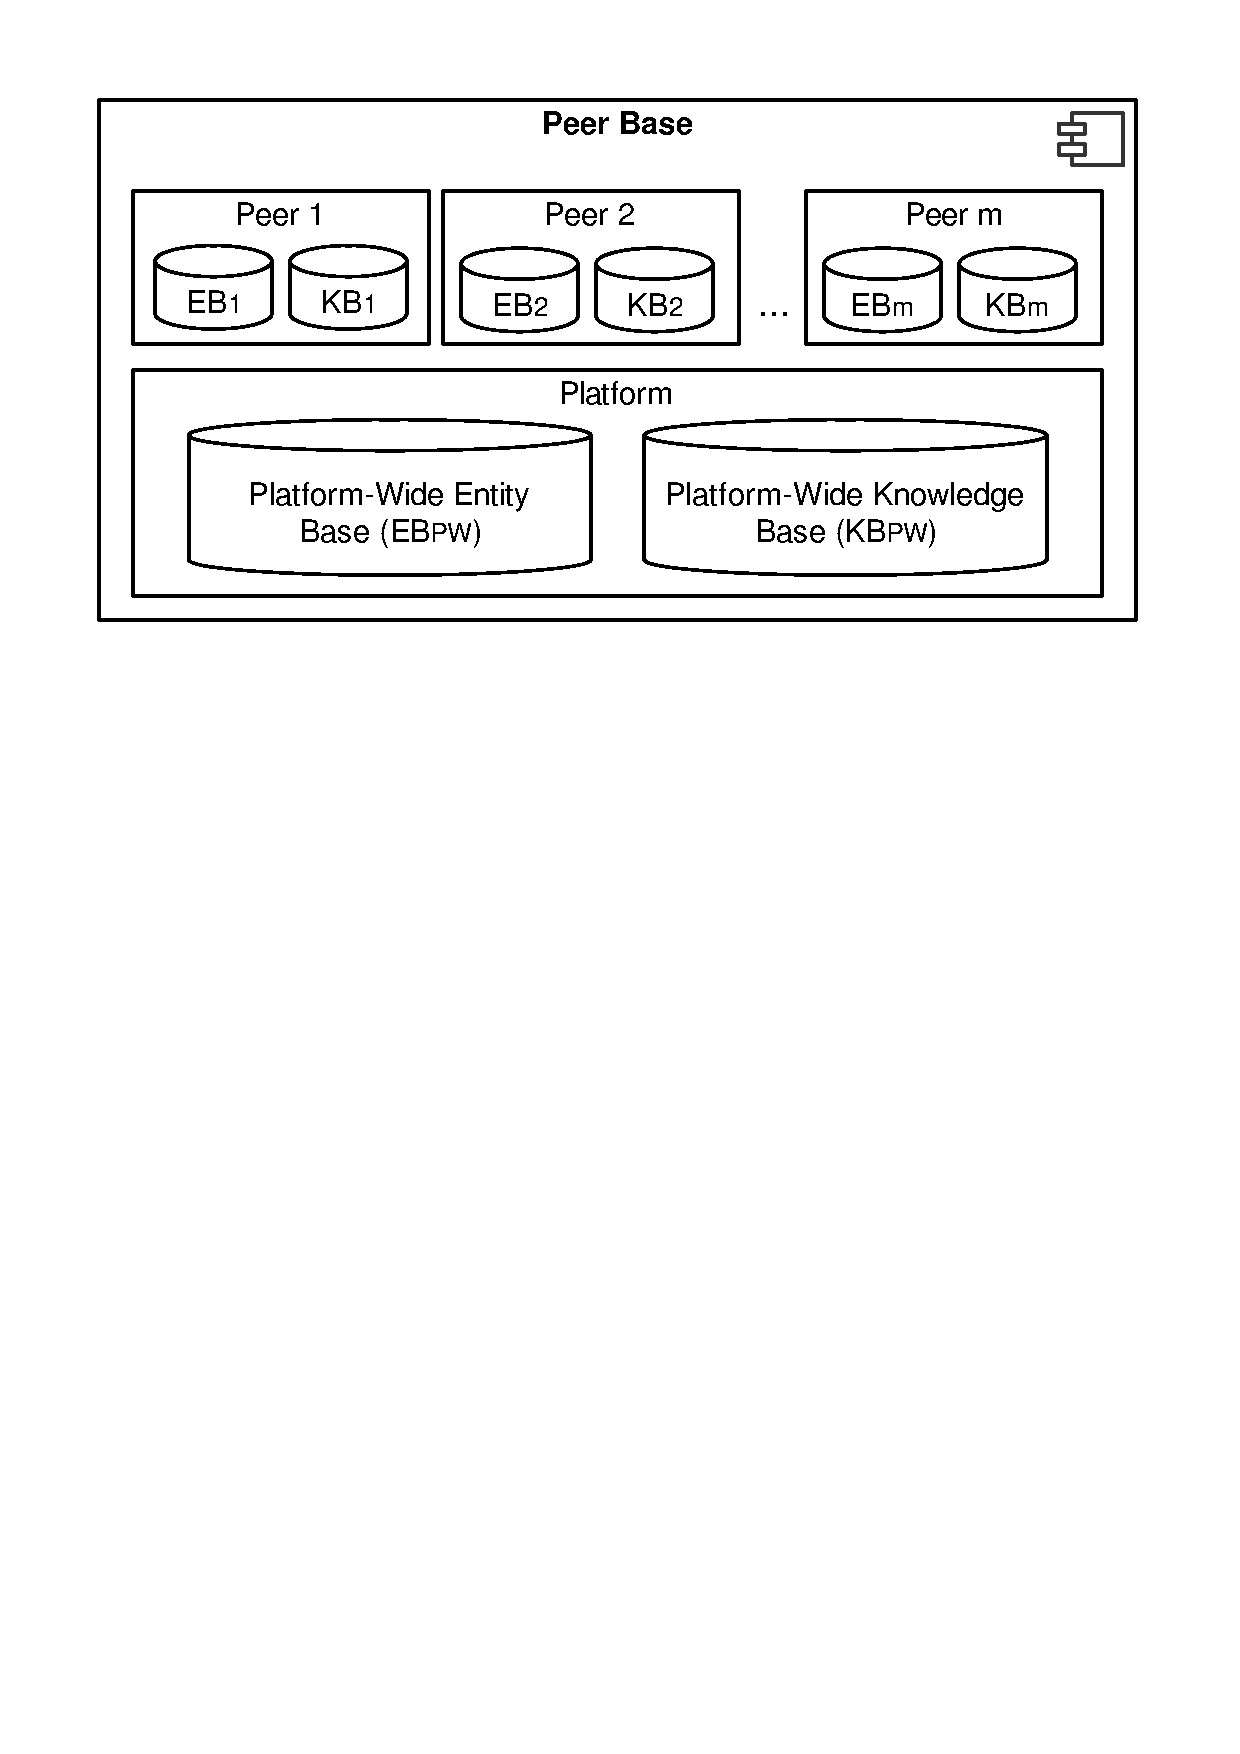
\includegraphics[width=0.65\linewidth]{figures/peerBase-diagram.pdf}
	\caption{Partial view of the Peer Manager internal architecture. Each subject its assigned its own peer storage, while the platform itself offers a shared Knowledge and Entity storages for different interactions.}
	\label{fig:peerManagerPlatform}
\end{figure}




\subsection{Implementation}
%{\it including how it has been implemented and specifications of APIs}

The Peer Manager component has been developed by following a three -layers approach, where each layer leverages the basic services offered by the level below and composes them for producing higher-level services. The resulting structure is shown in Figure~\ref{fig:pm-component-layers}; each layer will be further described in the remainder of this section. 

\begin{figure}[htbp]
\centering
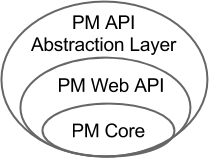
\includegraphics[width=0.3\textwidth]{figures/pm-component-layers.png}
\caption{Implementation layers of the Peer Manager}
\label{fig:pm-component-layers}
\end{figure}


\subsubsection{Peer Manager Core}
The Peer Manager Core provides a privacy-aware semantic storage for the SmartSociety Platform. This layer is implemented using Java, along with common data access frameworks like Spring and Hibernate.
While these technologies represent previous work from the University of Trento, the SmartSociety (through the work documented in~\cite{D1.1,D4.1,D4.2}) has created the Knowledge Model used for representing peers, users, profiles (i.e. personal information) and more generally managing the information for running an HDA-CAS.

No major changes have been done to the models or structures of the Peer Manager during the first half of Y-3 (so the research reported in previous deliverables still holds) but efforts to update these models to its final version will start in the second part of the year (as T1.4 restarts) and will have its results reported in Deliverable D1.3. No major changes are foreseen, so the underlying code and the exposed interfaces will likely be subject to minor revision only. 

\subsubsection{Peer Manager Web API} \label{ssec:pm-web-api}
This layer takes the Java classes that implement the Peer Manager Core and wraps them in HTTP API calls. 
No major changes to the APIs described in~\cite{D4.2} were introduced in Y-3. API specifications for this layer may be found in the Appendix~\ref{sec:pm-web-api-detail}.

\subsubsection{Peer Manager abstraction layer API} \label{ssec:pm-abs-api}
\todo{Content describing the purpose of this layer and the technologies used to implement it will be added to this section for the final version of this document}
 
This is a new component being developed specifically for the SmartSociety project and as such all code belonging to this layer will be open sourced. API Specifications for this layer may be found in the Appendix~\ref{sec:pm-abs-api-detail}.


\subsubsection{Integration with PPL policy language}
\todo{The content of this section needs to be refined}
\todo{Add a two-sentences description of what is PPL and its role in the overall PM functionality}
The integration process has been broken down in three incremental stages. 
% in three progressive steps or levels in order to better manage our development resources while complying with the SmartSociety project requirements.
%At each successive level both, the computational effectiveness of the achieved integration and the amount of work required, would increase. Nevertheless, the services offered by the integrated systems should remain mostly unchanged across the three levels of integration. 
\subsubsection{Basic Integration Approach - Decoupled Knowledge and Data}
\todo{Add A-PPL and Pii to the list of acronyms and define them}
In the first stage, for each of the profiles in the Peer Manager, A-PPL will have a corresponding Pii structure in its database. The overall structure is shown in Fig.~\ref{fig:pm-ppl-lv1.png}.

\begin{figure*}[htb!]
\centering
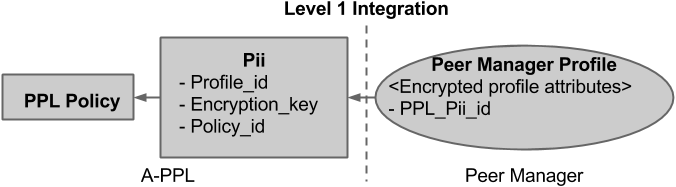
\includegraphics[width=0.8\linewidth]{figures/pm-ppl-lv1.png}
\caption{Basic Integration between the PM and PPL.}
\label{fig:pm-ppl-lv1.png}
\end{figure*}

It is important to note that the actual attribute information in the profile is not immediately accessible even to its owner (we may go as far as to encrypt it if necessary) and to read this information it needs to read the corresponding Pii entity stored in A-PPL (thus having to comply with the policy that protects the Pii).
\todo{Rephrase the next sentences and clarify what is *actually* delivered in the prototype}
Again, this is the simplest (but least effective way) to achieve integration and be absolutely sure that A-PPL authorizes the reading of the information in the Peer Manager Profile.
Of course there are issues to address, like having only a single unchanging encryption\_key for  each profile undermines purpose biding (you ask access to the info for one purpose and once granted access you can do whatever you want with the info, even use it for other purposes). Nevertheless, for Proof-of-Concept integration (and for this year's deliverable) I strongly believe this approach to be of enough value.

\subsubsection{Advanced Integration Approaches}
In the second stage of integration, the Peer Manager embeds knowledge of the inner details of PPL policies, so it is now able authorize the use of the information and store the information unencrypted, as shown in Fig.~{fig:pm-ppl-lv2.png}.

\begin{figure*}[htb!]
\centering
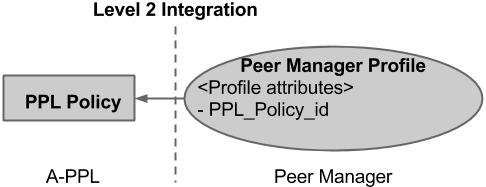
\includegraphics[width=0.6\linewidth]{figures/pm-ppl-lv2.png}
\caption{Advanced Integration between the PM and PPL.}
\label{fig:pm-ppl-lv2.png}
\end{figure*}

Note that the interaction with the A-PPL system is still used for the Policy storage (as the PM is supposed to have still no knowledge of how these policies are represented). Furthermore, the Peer Manager will still ask the A-PPL system if a requested operation complies or not with a given policy (as the PM does not share the same semantic ontology as A-PPL it cannot know if a request complies with a Policy even if it has all information about both structures).

In the final stage of integration the Peer Manager will represent a Policy as an Entity, and the A-PPL ontology used for reasoning about policies will be migrated to a specific and protected Knowledge Base in the Peer Manager.
With these two improvements, the Peer Manager will be able to support and enforce PPL without ever needing to call the A-PPL system. 


\subsubsection{Implementation of the Basic Integration Approach}
\todo{This is all in the future, so the Q is: what has actually been done so far?}
We will start with the level one integration, but in order to keep the generality we will make it possible to ask both about attributes and profiles. The profile will be treated as an ordinary attribute type. A profile is created for each purpose or combination of purposes needed.
In order to introduce the fact that an attribute is tied to one or more profiles and that encryption is needed the PIIType structure will be expanded with the fields profileID and encryptionData, encryption data in turn will consists of the fields  key, method and a list of parameters. Since no attribute type values are stored currently all attributes are considered to have a null value and the encrytionData is returned rather than the attribute value when the attribute type is retrieved.
In order to facilitate this the API of A-PPLE will be changed in the following way:
\begin{enumerate}
	\item We will add a structure containing profileID and encryption key in a many to one  relation to a PIITYPE. This will tie a list of profileID, encryptionData pairs to an attribute name and owner.
	\item We will construct a simpler version of the createPII call that do not require the sender to know about the PII type and also require profileID and encryptionData when storing and remove the attribute value since that is already stored in the PeerProfile.
	\item Since it can be cumbersome to make create calls for all attributes in a profile, if this should be needed we will violate the rest a bit and make a create call that takes a list of attributes and associated values and creates them in bulk. 
	\item We will change the getPII to require a profile id as well and to return encryptionData rather than the value of the attribute if it succeeds.
	\item  Like in 3 we will create a bulk call for retrieving multiple clearances and encryptionData for attribute names in bulk.
In the cases when just the profile attribute is used for clearance there we will have to need a ppl policy just containing the attribute name ”profile”, the profileID and the purpose covered by that profile. In order to do this the value (id) of that profile would have to be known when the policy is created so we would in have one specific policy for each profile. This ppl policy will however be fairly simple at the start and only differ in the profileID and purpose.
In order for A-PPLE and the Peer Manager to “understand” each other purpose names and attribute names needs to be aligned or known by both entities. 
\end{enumerate}

\section{Search, Matching and Ranking}
\label{sec:matching_ranking}
%\todo{ALETHIA - first draft by 30/May}

The search service provided by the Peer Manager (PM) was initially described in~\cite{D4.2}. In this deliverable we describe its evolution and provide more details about the meta-data models that are related with the search and ranking techniques, as well as their implementation.

\subsection{Mechanisms and algorithms}
%{\it including flow diagram, pseudo-code if needed, whatever explain how it works}

In order to select mechanisms and algorithms for implementing search in the PM we need to take into account existing approaches from the state of the art that can be used. For instance, there are many models and data structures that can be borrowed from the area of Information Retrieval (IR) as well as different matching techniques that can be used with different types of values. 

A logical view of the Search component is shown in Fig.~\ref{fig:search_diagram}, and presents the internal mechanisms, called subcomponents, that are integrated within the PM to deal with different types of queries (i.e., constraints on values of different natures). 
In what follows, these subcomponents are described in more details.

\begin{figure}[htbp]
\centering
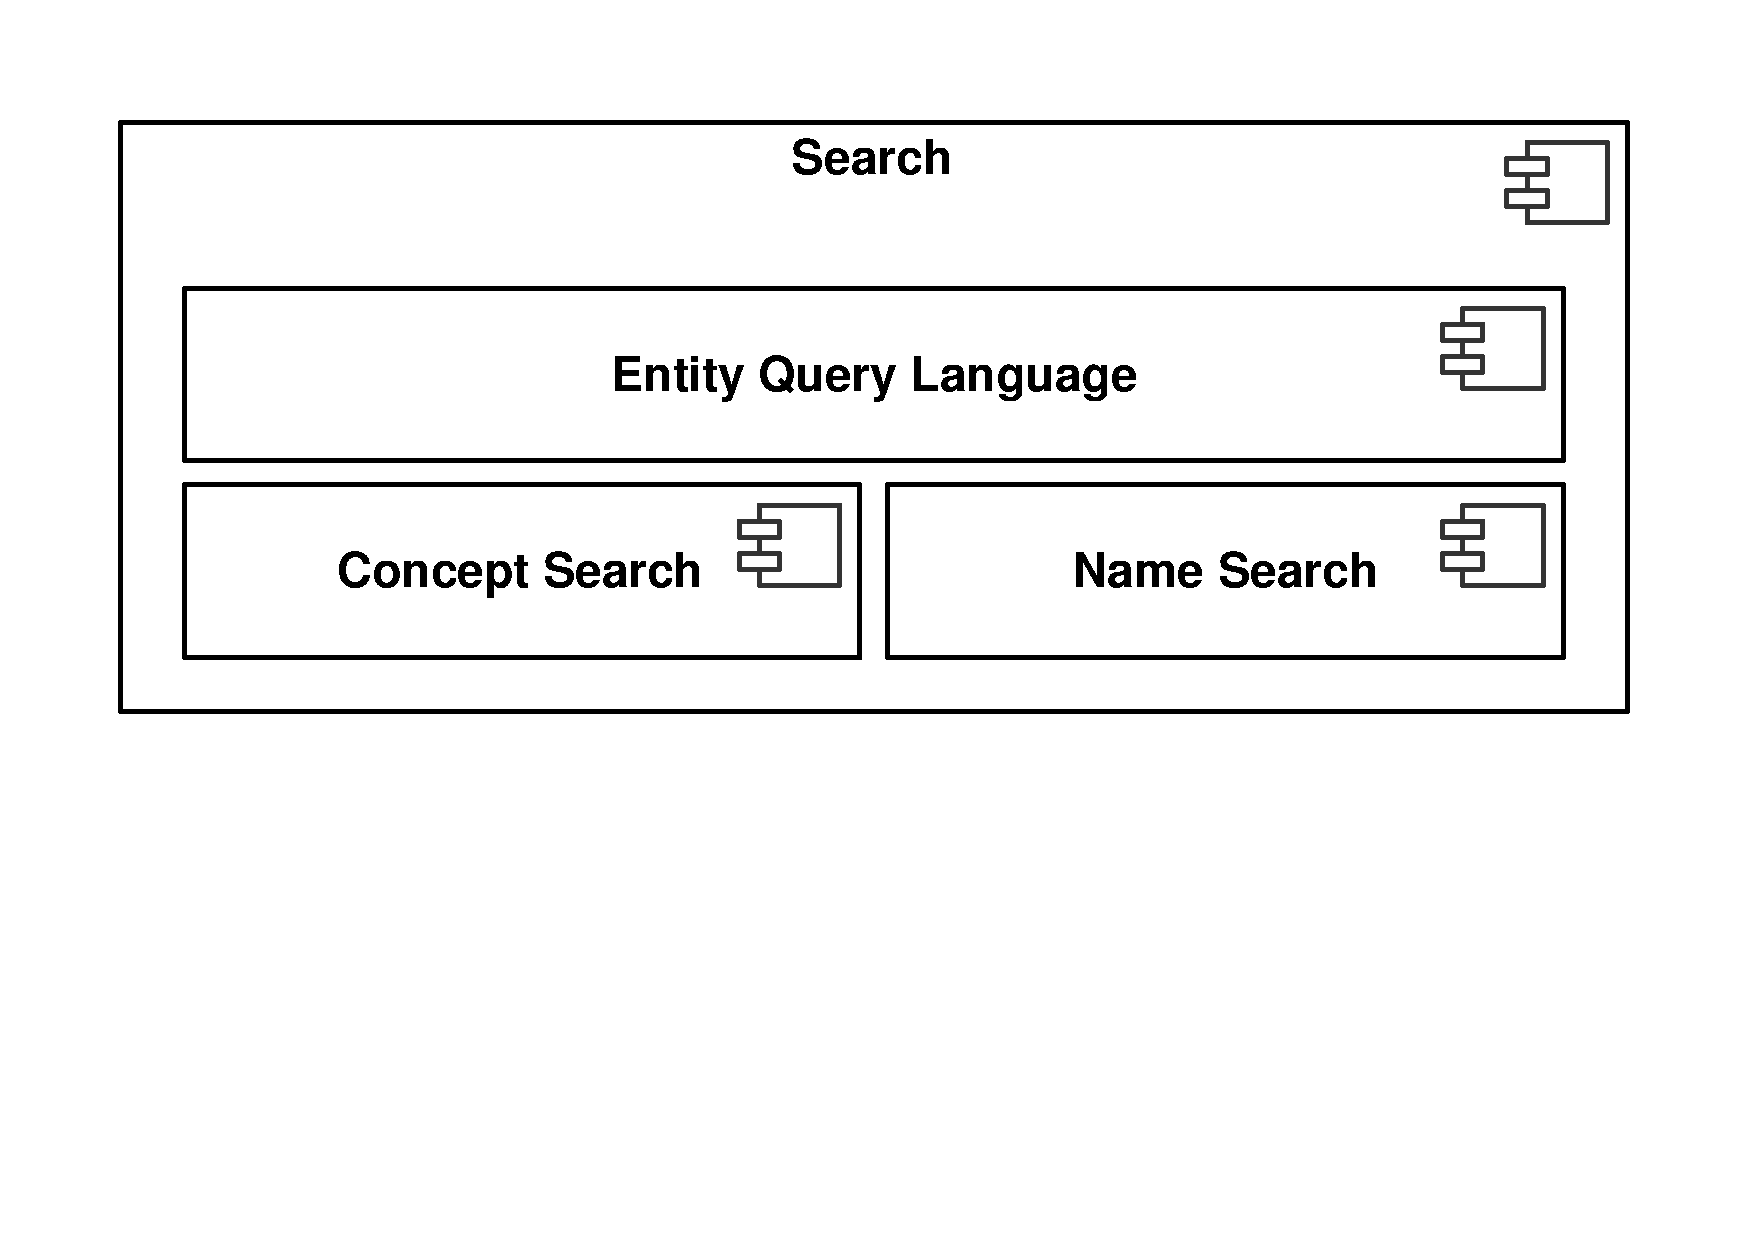
\includegraphics[width=0.65\textwidth]{figures/SearchComponentDiagram}
\caption{Search Diagram}
\label{fig:search_diagram}
\end{figure}

\paragraph{Concept Search.} 
\label{par:concept_search}
The lower part of Fig.~\ref{fig:search_diagram} shows two approaches that are used to deal with descriptions and names of peers. In particular, Concept Search, is used to match attributes from peers profiles with the search request. Concept Search~\cite{Giunchiglia:2009fk} was inspired by many syntactic IR systems that implement term matching by computing string similarity between words. For example, search for identical (possibly stemmed) words, words with common prefixes, words within a certain edit distance with a given word, or words that sound similar (see~\cite{Manning:2008:IIR:1394399} for more details on existing syntactic search approaches). 

However, when trying to match peer's attributes with a search query in the PM, there are many problems related with syntactic IR systems that can negatively affect the quality of search results. In particular, we know that different words can have the same meaning (synonymy); the same word may have multiple meanings (polysemy); and the meaning of words can be different but still semantically related. To deal with these problems, Concept Search extends the syntactic search approach with semantic search. In this approach, the retrieval models and data structures of syntactic search are reused. The main difference is given by the fact that concept search leverages on the core semantic data model of the PM and therefore concepts are used as terms instead of words. As a consequence, term matching is implemented by using semantic matching of concepts~\cite{Giunchiglia:2007ve}. On the other hand, when the semantic information is not available (i.e., when the concepts of a given set of words cannot be computed), words are used as terms and concept search falls back to the underlying syntactic search.


\paragraph{Name Search.} 
\label{par:name_search}
When dealing with peers that can be humans, it is important to account for the relevance of human readable identifiers (i.e., names). 
Names are labels composed by a combination of words, numbers and symbols. They are different from other attributes because they play the role of keywords rather than been mapped to concepts from a knowledge base. 
A name search algorithm deals with the problem of finding all the possible candidate entities that have names equal or similar to a given name.

Names can suffer from different types of variations, such as, format variations (e.g., \emph{George Augusto Lombardi} vs. \emph{George A. Lombardi} vs. \emph{Lombardi, George}), translations (e.g., \emph{Trento} in Italian vs. \emph{Trient} in German vs. \emph{Trent} in English), or misspellings (e.g., \emph{Fausot} vs. \emph{Fausto} vs. \emph{Fuasot}). These name variations show the complexity with which a name search algorithm has to deal. Various syntactic search techniques can be used for implementing name search. 

In the name search algorithm implemented by the PM, the following techniques are applied in a sequential order until the entities with the matching names are found:
\begin{inparaenum}[(i)]
\item \emph{Exact matching} between a given name and the entity name; 
\item \emph{Fuzzy search} techniques are employed by comparing name tokens using, for instance, jaccard~\cite{Bilenko:2003pd} similarity coefficient for comparing the similarity\footnote{\url{http://en.wikipedia.org/wiki/Similarity_measure}} of token sets.
\item Prefix search technique is used to perform fuzzy search on tokens themselves to account for the fact that, according to~\cite{Pollock:1984rr}, fewer errors usually occur at the beginning of names. 
%Search for name tokens having the same prefix can be efficiently implemented both in the inverted index vocabulary and by using SQL like queries.
\item Finally, the trigram search technique (N-gram index with grams of length 3) is used to account for the case of misspelled names. The pg\_trgm\footnote{\url{http://www.postgresql.org/docs/8.4/static/pgtrgm.html}}  module from PostgreSQL database management systems is used to implement trigram search on entity names in the current implementation. 
\end{inparaenum}


\paragraph{Entity Query Language.} 
\label{par:entity_query_language}
The upper part of the figure shows a subcomponent that builds on the two types of searches presented above and supports additional search operations based on the relations between entities. An Entity Query Language (EQL) provides more flexible and heterogeneous language to access peer’s attributes as well as additional operations. 
EQL is used by the PM to extend the low-level mechanisms. It can be seen as a semantically enabled version of HQL\footnote{\url{http://docs.jboss.org/hibernate/core/3.3/reference/en/html/queryhql.html}} on entities, where HQL is an object-oriented query language similar to SQL. More details about EQL are provided in the Annex~\ref{sec:search-annex}.


\subsection{Implementation}
%\todo{how it has been implemented} 

The Peer Manager's implementation of its search service (search, matching and ranking services) uses Java in combination with Hibernate and Spring frameworks, a PostgreSQL database is used for storage of peers' information and profiles. The Peer Manager front-end uses NodeJs and exposes its basic search functionalities through a low level HTTP API. In order to facilitate the interaction with other SmartSociety components (also in light of specific prototypes and demos), the PM provides also a high level API that results in more powerful and easy-to-use calls. Such calls leverage the full power of the Peer Manager and allow other components to abstract from internal details related to the PM's implementation. 

It is important to note that the implementation of the underlying mechanisms at the core of the PM's search implementation represent previous knowledge/work of the University of Trento Knowdive research group, so its source code will not be made commonly available. However, the full source code of the high level API corresponding to the front-end implementation that is specific for SmartSociety will be made available as part of the project. In the rest of this section we provide more details on how to use the search service, which in turn is related with the implementation of the high level API. 

\subsubsection{Search Service}\label{subsec:concept_search}
%\todo{documentation of search service including syntax/examples of EQL}

The Concept Search approach is used by the PM to implement concept based search on attributes from peers profiles.
The syntax of attribute-based concept search queries is designed to be similar to the query syntax of Lucene\footnote{\url{http://lucene.apache.org/core/old_versioned_docs/versions/3_5_0/queryparsersyntax.html}}, a popular Java based open-source indexing and search library. The current implementation supports concept search on attribute values, e.g. the query \emph{``big restaurant''} among other results will also return entities with attributes containing phrase \emph{``huge steakhouse''}. Concept search is also implemented on top of attribute names, e.g. the entity with attribute \emph{``location:Trento''} will be returned as an answer to query \emph{``place:Trento''}. Atomic queries on attribute values and attribute names can be combined into more complex queries by using Boolean operators, e.g. \emph{``big restaurant AND location:Trento''}.

The more flexible access to search services can be exploited through the specification of a search query using EQL language. The current implementation of the PM's search service supports only a subset of HQL, however, new features will be added if (and when) needed. The EQL implementation currently used in the PM supports the FROM clause, allowing the simplest query specification, as well as the SELECT, JOIN, GROUP BY, WHERE, and ORDER BY clauses that allow the specification of more complex queries. Among them, the ORDER BY clause is of key importance because is the one that is used to implement the ranking of search results. 

Note that concept search is used within FROM and SELECT clauses, which means that there is no need to know the exact name of the entity type or attribute name. Concept search approach is used for matching entity types in \emph{from} clauses and attribute names in \emph{select} clauses. 
 For instance, in the case when there is a synonymy relationship between concepts \emph{restaurant} and \emph{bar} in the underlying knowledge base, the search to find all the restaurants can also be performed by using the query ``\texttt{FROM bar r}''.

Another use of concept search query in \emph{from} clause can be to select a subset of all the entities for a given entity type. 
This is done by adding additional constraints, using concept search syntax, into the \emph{from} clause.
For instance, in the query ``\texttt{FROM bar [description:steakhouse] r}'', the additional constraint ``\texttt{[description:steakhouse]}'' requires that descriptions of found bar entities contain concepts which are more specific than the concept `steakhouse'. This means that a description containing `steakhouse in Trento' would comply with such requirement and the corresponding entity can be included in the search result. 
%\todo{Last sentence unclear, please clarify example}


%%%%%%%%%%%%%%%%%%%%%%%%%%
%%%%%%%%%%-Limitations-%%%%%%%%%%
%%%%%%%%%%%%%%%%%%%%%%%%%%

%On the other hand, the current limitations include:
%\begin{enumerate}
%\item \textbf{Joins:} Only inner join is supported, i.e., the keyword \emph{join} is used for specifying inner join.
%\item \textbf{Nulls:} If an attribute name is selected, then only NOT NULL attribute values will be returned.
%
%\begin{tabular}{ll}
%\texttt{SELECT cat FROM Cat cat} & [all cats will be found] \\
%\texttt{SELECT cat, cat.name FROM Cat cat} & [cats without names will be skipped] \\
%\end{tabular}
%\item \textbf{Aggregates:} Only simple aggregate functions on attributes are supported, e.g. count(cat).
%\item \textbf{Dots:} As in HQL, dot-notation is used for accessing entity attributes. There are limitations on how dots are used. The first (and only the first) dot defines an attribute (e.g. cat.name). The second dot can be used only for accessing the meta-data (e.g. cat.name.metadata). Note, that it is not really a limitation because all the queries with two or more dots can be rewritten by using explicit joins, as it is shown below:
%
%\begin{tabular}{p{0.45\textwidth}p{0.45\textwidth}}
%\texttt{SELECT cat.mate.name} & [not supported] \\
%\texttt{FROM Cat cat} & \\
% & \\
%\texttt{SELECT mate.name}  & [equivalent query with explicit join] \\
%\texttt{FROM Cat cat} & \\
%\texttt{JOIN cat.mate mate} & \\
%\end{tabular}
%\end{enumerate}


%%%%%%%%%%%%%%%%%%%%%%%%%%
%%%%%%%%%%-Additional notes-%%%%%%%
%%%%%%%%%%%%%%%%%%%%%%%%%%

%Additional notes:
%\begin{itemize}
%\item If no attribute is specified in select or where clause, entity id is used as a default attribute. For instance, 
%``\texttt{SELECT cat FROM Cat cat}'' internally, will be translated to ``\texttt{SELECT cat.id FROM Cat cat}''
%
%\item Specifying an alias (e.g. cat) is required. For instance, ``\texttt{FROM Cat cat}''
%
%\item If concepts with multi-words are used for defining types or attributes, spaces between words should be replaced with underscore `\_'. For instance, ``\texttt{SELECT cat.first\_name FROM Cat cat}''.
%
%\item Underscore `\_' can also be used for specifying correct concepts which should be used for attribute names and types. For instance, ``\texttt{SELECT cat.name\_123 FROM Cat\_321 cat}''.
%\end{itemize}
%


\subsubsection{Main Search Endpoint Documentation}
%\todo{The specification of the search APIs with an example will be added here for the final version of this document.}

The Table~\ref{tab:searchApi} shows the specification of the search API and a simple example of the call and response for searching all available peers for a generic task. 

\begin{table}[htdp]
\caption{Search API}
\begin{center}

\begin{tabular}{|l|l|p{9cm}|}
\hline
\textbf{Method} & \textbf{Api} & \textbf{Description} \\
\hline
GET & 
instances/search & 
Returns a set of entity instances that match with the characteristics specified in the input query. In the example, the call is used to obtain a list of users representing peers that matches with a set of requirement. \\
\hline
\multicolumn{3}{|c|}{\textbf{Call Example}} \\
\hline
\multicolumn{3}{|p{14cm}|}{
\url{
http://demos.disi.unitn.it:8080/smartsociety-score-api/instances/search?query=select\%20user1\%20from\%20User\%20user1\%20join\%20user1.entity\%20person1\%20where\%20person1.available\%20\%3D\%20true\&entityBase=5408\&instanceClass=Instance\&queryType=\%20EQL\&parseSemantics=false\&includeExplanation=false\&includeCount=false\&idsOnly=false\&pageIndex=1\&pageSize=10\&maxDepth=1\&includeSemantics=false\&maxValues=10\&includeAttributes=false\&createAttributeMap=false\&attributeFilterType=ATTRIBUTE\_DEF\_ID\&includeAttributesAsProperties=false\&includeTimestamps=false
}}
\\ 
\hline
\multicolumn{3}{|c|}{\textbf{Response Example}} \\
\hline
\multicolumn{3}{|p{14cm}|}{
\{
  ``@type'': ``EQLSearchResult'',
  ``results'': [
      [``6604''],
      [``6605''],
      [``6606'']
  ]
\}
} \\
\hline
\multicolumn{3}{|c|}{\textbf{Response General}} \\
\hline
\multicolumn{3}{|p{14cm}|}{
\{
  ``@type'': ``EQLSearchResult'',
  ``results'': [
      [``\textcolor{ao(english)}{$\langle$ Returned userId 1$\rangle$}''],
      \textcolor{ao(english)}{\ldots}
      [``\textcolor{ao(english)}{$\langle$ Returned userId N$\rangle$}'']
  ]
\}
} \\
\hline


%\multicolumn{3}{|l|}{\{} \\
%\multicolumn{2}{|l}{``@type'': ``EQLSearchResult'',} & \\
%\multicolumn{2}{|l}{``results'': [ } \\
%\multicolumn{3}{|l|}{ [``6604''],} \\
%\multicolumn{3}{|l|}{ [``6605''],} \\
%\multicolumn{3}{|l|}{ [``6606''] } \\
%\multicolumn{3}{|l|}{ ] }\\
%\multicolumn{3}{|l|}{\}} \\
%\hline
\end{tabular}

\end{center}
\label{tab:searchApi}
\end{table}%





















%\section{Privacy-preserving Measures}
%{\it here goes all discussion on how the current implementation supports privacy, what is missing and when -and if- it will be delivered}
% 
%\todo{this section could be removed because the privacy preserving measures are embedded in sections \ref{sec:profiling} and \ref{sec:matching_ranking}}

\section{Evaluation Plans}
\label{sec:evaluation}
%\todo{RONALD and ALETHIA}

%{\it including assessment against functional requirements - elicited from use cases - and performance measures based on the actual  deployment}
  
  
\todo{this section contains preliminary content}

%Intro to evaluation
\todo{missing section introduction}
%Privacy and security as a second concern

\subsection{Analytic Validations}
The analytic part of the validation include formal or semi-formal validations and analysis of the different properties of the system. This validation tests will be interested, in particular, in comparing the implemented version of the Peer Manager with its ideal counterpart described during the first and second year deliverables (requirement compliance) and also finding out ``the cost of privacy'' by calculating the overhead in time and space that implementing these privacy measures brings to general systems.

The first results of this analytic validation activities will be reported during the third year review meeting of the project with the final results reported in D4.4 and the fourth year review meeting.

\subsubsection{Requirement compliance}
The requirement compliance of the peer manager comprises both evaluation of the general project requirements (found in the DoW and in D1.1??) and the compliance with the privacy requirements established in D4.1 and revised in D4.2.

For the compliance with the privacy requirements we plan to express a simplified version of the Peer Manager using the formalization of privacy sensitive systems found in [??]. We will then proceed to prove the extent to which the so represented Peer Manager is in fact compliant with the privacy requirements set in earlier version of this deliverable. 

The strategy for validation of the project requirements will include applied methods such as unit and integration tests of the Peer Manager implementation; along with performance tests of the integrate Peer Manager as part of the project's use cases. For the last case, performance evaluations in both time and space will also be performed and reported accordingly.  

\subsubsection{``Cost of privacy'' measurements}
This exercise will compare the time and space complexity of two Peer Managers, one without any privacy considerations and the other (as developed for the project) compliant with the set privacy requirements. Generalizing one step further, it is expected that this comparison would be able to show an estimate of the cost in time and space complexity for complying with these privacy requirements (that are now part or being discussed to become part of the EU privacy legislation) in a wide-range of relevant systems.

More in particular, the time/space complexity in both the privacy-less and the privacy-enabled Peer Managers will be compared independently for storing information and reading/accessing this information, 

\subsection{SmartShare Exploratory Survey}
SmartShare is a ridesharing application developed by the SmartSociety consortium as test and validation of several of the project's ideas.  A trial using the SmartShare application is planned during the second half of 2015 in multiple Italian municipalities.  

As part of the SmartShare trial, we plan to carry out an exploratory survey aimed initially to gauge the interest and knowledge of the participating users in privacy-related issues and technologies. Furthermore, based on these results we plan to adjust and create requirements related to the focused user activities and testing planned for year four.
 
The list of the questions being asked in this exploratory survey can be found in the Appendix~\ref{sec:smartshare-survey} and the results of this validation activity will be reported during the third year review of the project.

\subsection{Usage analysis of the SmartSociety Platform}
Through integration with the SmartSociety platform the peer manager will be used in several of the small-scale experiments organized by WP8 and also the Virtual Gamified Environment developed as part of WP9. We will take these opportunities to measure the real-use performance of the Peer Manager and, when possible, get information from the involved users.

\todo{Specific questions to be asked by WP4 towards the Virtual Gamified Environment to be added here}

The results of this validation activity will be part of the D4.4 and will be reported during the fourth year review of the project.

\subsection{Focused user activities and testing}
The final focused user activities relating to the peer manager and platform-wide privacy considerations will be carried out during the fourth year of the project. We plan to use all previous validations (specially the SmartShare Exploratory Survey) to inform and better adjust this validation activity. 

Based on this, further quantitative and qualitative user-related studies may be carried out, already aiming to validate not only the Peer Manager but also to draw project-wide and CAS-related conclusions of the exercise. 

The results of this validation activity will be part of the D4.4 and will be reported during the fourth year review of the project.


\section{Integration}
\label{sec:integration}
The Peer Manager has been integrated in the SmartSociety platform
during the second year of the project, and released as component of
the version 1.0 of the platform. 

Currently the Peer Manager functionality
is used in both project-wide scenarios, i.e., SmartShare and
AskSmartSociety!~\cite{D8.2,D8.3}.

In general terms, the PM is mostly used as privacy-preserving
information service for peer-related information. In this sense, it is
at the center of a rather complex web of interactions with other
components. In particular, it is used by the Orchestration Manager to
identify suitable peers for carrying out a given task (composition
phase). It also provides information on how peers shall be contacted
for the negotiation process, the actual interaction being mediated by
the SmartCom middleware. The PM is tightly interacting with the
Context Manager, a component (developed within WP3) able to mine
streams of data to provide a near real-time representation of the
current user context. This situational information is integrated as
dynamic part of the user profile, and can be used for ensuring the
search process returns purposeful results. 

In this section we briefly describe how the PM is used in the context
of overall SmartSociety platform architecture, with reference to the
two aforementioned scenarios.

In both contexts, the PM is used to perform all operations related to
the management of collectives
(creation, retrieval of peers in a collective and retrieval of peer
information and contact method for communication
purposes~\cite{D8.2}). In SmartShare a collective is the set of peers
representing users taking part in a ride. In AskSmartSociety! a
collective is the set of peers selected as adequate (by the PM) to
answer a given question. These operations are typically requested by
the application peer (creation of collective) and by the SmartCom
communication middleware (retrieval of peers in a collective and peer information).

The PM search functionality plays a key role in the AskSmartSociety!
application scenario, where it is exploited to identify a suitable set
of peers who could best contribute to answer a given
question. This function is invoked by the OM and the response triggers
the execution of the negotiation process~\cite{D8.2}. In the context
of AskSmartSociety!, the ability of
the PM to handle transparently machine and human peers represent a key
feature, in that it enables full hybridity of the application. Also, the usage of the Concept Search approach, and in
particular the ability of the PM to perform semantic matching on
peers' attributes is instrumental in identifying human peers with the
right expertise to answer a given query, hence contributing
significantly to the quality of the answers collected.


\section{Conclusions}
\label{sec:concl}
This deliverable included the description of  a number of key aspects related to the PM design, implementation and validation. 
In particular, it included:
\begin{itemize}
\item The mechanisms and implementation details for the profile schemas and the privacy-enhancing technologies used by the PM;
\item The mechanisms and implementation details for the services that allow searching, matching and ranking of peers based on different attributes (i.e., characteristics) from their profiles;
\item The evaluation plans for the PM including analytical and user-based evaluations; and
\item The description of how the PM is currently integrated in the SmartSociety platform and used in different project-wide scenarios.
\end{itemize}
In the second half of 2015 the focus will be on the validation of the PM functionality and performance, following the strategy outlined in Sec.~\ref{sec:integration}. At the same time, feedback from empirical activities in WP8 and WP9 will be used to fine-tune the PM APIs and the underlying mechanisms, with particular emphasis on search and ranking functionality. The final PM design and implementation will be shipped with D4.4 at M42.

%%%%%%%%%%%%%%%%%%%%%%%%%%%%%%%%%%%%%%%%%%%%%%%%%%%%%%%%%%%%%%
\newpage

%%%%%%%%%%%%%%%%%%%%%%%%%%%%%%%%%%%%%%%%
%%%%%%%%%%%%%%%%%%%%%%%%%%%%%%%%%%%%%%%%%%%%%%%%%%%%%%%%%%%%%%%%%%%%%%%%%%%%%%%%%%%%%%%%%%%%%%%%%%%%%%%%%%%%%%%%%%%%%%%%
\bibliographystyle{./IEEEtran}
\bibliography{BIB/biblio.bib}
\clearpage
\appendix
\section{SmartShare survey questions} \label{sec:smartshare-survey}
The following is a set of questions that form part of WP4's exploratory survey. Notice that because of the generality of these questions and how early they are presented within the evaluation strategy presented in Sec.~\ref{sec:evaluation}, rather than a full evaluation exercise (from which results for WP4 or the project may be extracted) this is more of an exploratory survey aimed to inform and adjust further evaluation activities.

\emph{First part.}
%Post-questionnaire for evaluating PETs

\begin{enumerate}
\item How much time will you spend at configuring / learning the system? 
	\begin{itemize}
	\item Very little
	\item Some time
	\item Lot of time, I like to understand every detail and be in control
	\item other: 
	\end{itemize}
\item In your opinion, was your data well protected when you tried to achieve a task? 
	\begin{itemize}
	\item Yes
	\item I wasn't concerned about that
	\item No
	\item other:
	\end{itemize}
\item Are you comfortable with the information that others find out about you when you tried to achieve a task? 
	\begin{itemize}
	\item No, I want to be completely anonymous
	\item Partially, I would like to share less information
	\item Yes, it was fine
	\item I might easily share more information to allow drivers/commuters to know me better
	\item other:
	\end{itemize}
\item Were you aware of who has access to your information after you completed the task?
	\begin{itemize}
	\item Yes
	\item No
	\item other:
	\end{itemize}
\item How secure, in relation with security of your information, do you feel after having completed the task? 
	\begin{itemize}
	\item Very secure
	\item Secure, I trust the system
	\item I wasn't concerned about that
	\item Insecure
	\item Very insecure 
	\end{itemize}
\end{enumerate}
	

\emph{Second part}
%PET-USES questionnaire

Please use the scale below to show to what extent you disagree or agree with the statements that follow.
\begin{enumerate}
\item Strongly disagree
\item Disagree
\item Neither agree nor disagree
\item Agree
\item Strongly agree
\end{enumerate}

\begin{itemize}
%Data Management
\item I get a clear view of my personal data from the system [~~~]
\item I find managing and organising my personal data easy with this system [~~~]
\item I find keeping track of various usernames and passwords is easy with this system [~~~]

%PrivPrefs
\item I find easy to use the settings for how much or how little data to be released with this system [~~~]
\item I will  find useful if the system helps me understand the effects of different privacy settings [~~~]
\item I would feel safer if I know that I will be notified by the system when I'm about to release more personal data than my chosen preference [~~~]

%Data Release
\item I know what personal information I'm releasing when I’m using this system [~~~]
\item I like to have control over how much or how little data to release in a given transaction [~~~]
\item The system makes it easy to decide how much or how little data to release in a given transaction [~~~]
\item It is clear from the system to understand who will receive my data [~~~]

%History
\item I can easily find out who has received my personal data with this system [~~~]
\item I want to get a good view of who knows what about me from this system [~~~]
\item I can easily see how much I’ve used a particular user name with this system [~~~]
\end{itemize}


\newpage
\section{Peer Manager abstraction layer API} \label{sec:pm-abs-api-detail}
The following document specifies the calls that the Peer Manager Year3 Proof of Concept accepts and the replies (example+format) that it produces.
This is a work in progress, new calls may be added but the already specified calls should remain stable

\subsection{Creation of a new Peer}
This call will create a peer structure, its corresponding main entity (based on the peer\_type argument) and a user structure (with the given username) linked to the peer. 
CALL format

\begin{figure*}[htb!]
\centering
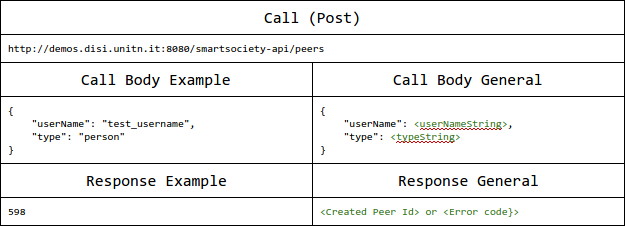
\includegraphics[width=1\linewidth]{figures/abs-new-peer.png}
\label{fig:abs-new-peer}
\end{figure*}

PARAMETERS
\begin{itemize}
	\item userNameString(required): alphanumeric string containing an unique username
	\item typeString(required): one of the following strings "human", "software"
\end{itemize}

POSSIBLE ERROR RETURNS (to be finalized)
\begin{itemize}
	\item NAME\_TAKEN: the provided username was already taken in the system
	\item INVALID\_TYPE: the provided type is not supported
\end{itemize}

\subsection{Update Peer Information}
This call updates the information in the main entity of the recently created peer.

\begin{figure*}[htb!]
\centering
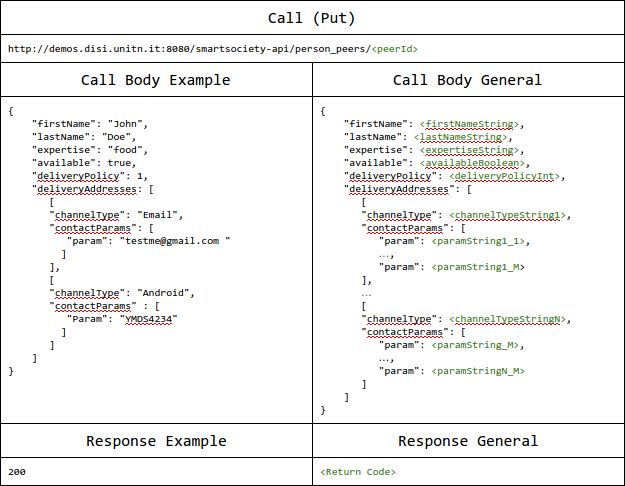
\includegraphics[width=1\linewidth]{figures/abs-update-peer.png}
\label{fig:abs-update-peer}
\end{figure*}

PARAMETERS
\begin{itemize}
	\item peerId (required - part of the call): id of the peer to update
	\item firstNameString(required): alphanumeric string containing first name of the represented person 
	\item lastNameString(required): alphanumeric string containing last name of the represented person
	\item expertiseString alphanumeric string (parsed later to a concept) that denotes the particular expertise of this person
	\item availableBoolean(required): boolean value that codifies if this peer is available for answering requests
	\item deliveryPolicyInt(required): integer value that codifies whether to deliver the message to one or more defined delivery Addresses (see SmartCom for the meaning of values, no validation done in the PM).
	\item channelTypeStringX(at least one required): string value that codifies the type of the communication channel  (see SmartCom for the meaning of values, no validation done in the PM)
	\item paramStringX\_Y(at least one required): string value that codifies a parameter that is useful for the current delivery address (e.g. the email address for an email type delivery address)
\end{itemize}

POSSIBLE ERROR RETURNS (to be finalized)
\begin{itemize}
	\item OK: peer updated without problem
	\item NOT\_A\_PERSON: the identified peer does not have a person main entity
	\item DATA\_INVALID: there was a problem processing the call body
\end{itemize}

\subsection{Create a SmartAsk Expert Profile}
This call updates creates a SmartAsk Profile for a given user\_id, this denotes that the user is in fact granting permission to SmartAsk to use the information contained in the profile.

\begin{figure*}[htb!]
\centering
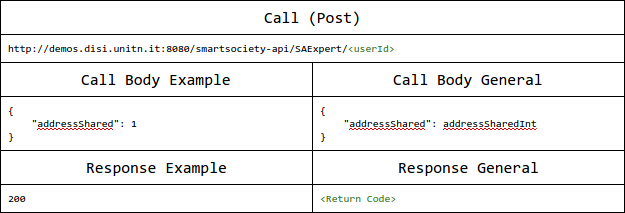
\includegraphics[width=1\linewidth]{figures/abs-new-profile.png}
\label{fig:abs-new-profile}
\end{figure*}

PARAMETERS
\begin{itemize}
	\item user\_Id (required - part of the call): id of the user of which to create the SAExpert profile
	\item addressShared: order of the delivery address that wants to be included in the created profile (1 means the first one defined, 2 the second, and so on). Defaults to 1
\end{itemize}

POSSIBLE ERROR RETURNS (to be finalized)
\begin{itemize}
	\item OK: profile created without problem
	\item INVALID\_USER: there user id was not found or does not belong to the authenticated user.
	\item INVALID\_ADDRESS: the address number was not defined
\end{itemize}

\newpage
\section{EQL details} \label{sec:search-annex}
%\todo{ALETHIA - first draft by 30/May}

%The search service provided by the Peer Manager (PM) was initially described in deliverable D4.2~\cite{D4.2}. In this deliverable we describe its evolution, by providing more details about the meta-data models that are related with the search and ranking techniques, as well as their implementations.
%
%\subsection{Mechanisms and algorithms}
%
%In order to select mechanisms and algorithms for implementing search in the PM we need to take into account existing approaches from the state of the art that can be used. For instance, there are many models and data structures that can be borrowed from the area of Information Retrieval (IR) as well as different matching techniques that can be used with different types of values. 
%%It is also important to define what is the atomic element (term) that will be used in the data and query representations.
%
%A logical view of the Search component is shown in Figure~\ref{fig:search_diagram}, and presents the internal mechanisms, called subcomponents, that are integrated within the PM to deal with different types of queries (i.e., constraints on values of different natures). 
%In what follows, these subcomponents are described in more details.
%
%In particular, the lower part of the figure shows two approaches that are used to deal with descriptions and names of peers. The upper part of the figure shows a subcomponent that builds on the other two to provide more flexible and heterogeneous language to access peer’s attributes as well as to provide additional operations. 

%\begin{figure}[htbp]
%\centering
%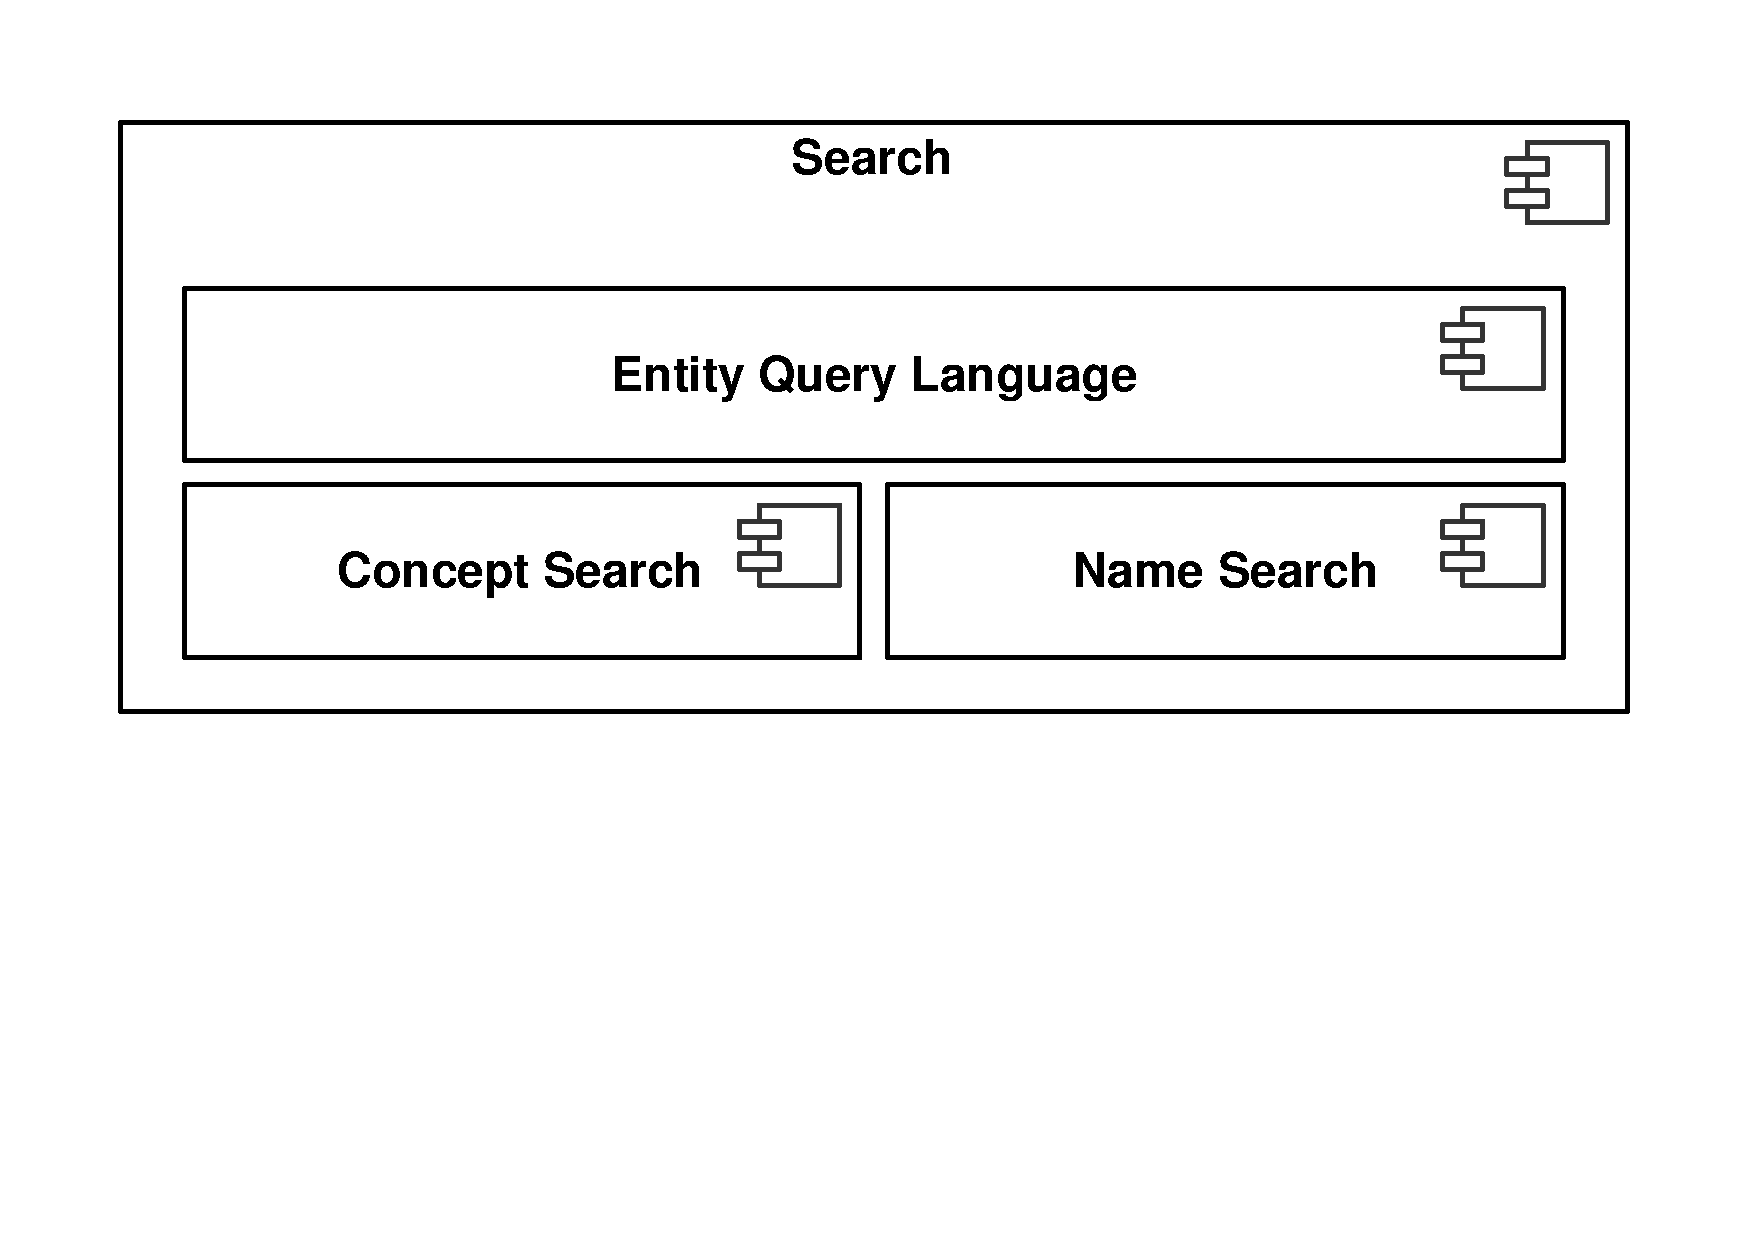
\includegraphics[width=0.65\textwidth]{figures/SearchComponentDiagram}
%\caption{Search Diagram}
%\label{fig:search_diagram}
%\end{figure}


%\subsubsection{Concept Search}
%\label{subsec:concept_search}
%Among existing IR models we can find the classical example of the vector space model that is used for computing query answers and relevance ranking. Among the different data structures used in IR systems, a widely used example for implementing efficient indexing and retrieval is the inverted index (also referred to as postings file or inverted file)\footnote{\url{http://en.wikipedia.org/wiki/Inverted_index}}. Next, we need to define the atomic element and the matching techniques to be used. 
%Many syntactic IR systems implement term matching by computing string similarity between words. Some examples of how term matching can be implemented are search for identical (possibly stemmed) words, words with common prefixes, words within a certain edit distance with a given word, or words that sound similarly (see~\cite{Manning:2008:IIR:1394399} for more details on existing syntactic search approaches). When trying to match peer's attributes with a search query in the PM, we consider also many problems that can negatively affect the quality of search results. In particular, we know that different words can have the same meaning (synonymy); the same word may have multiple meanings (polysemy); and the meaning of words can be different but still semantically related.

%In order to deal with these problems from syntactic information retrieval approaches, the PM uses Concept Search~\cite{Giunchiglia:2009fk} that extends the syntactic search with semantic search. In this approach, the retrieval models and data structures of syntactic search are reused. The main difference is given by the fact that concept search leverages on the core semantic data model of the PM and therefore concepts are used as terms instead of words. As a consequence, term matching is implemented by using semantic matching of concepts~\cite{Giunchiglia:2007ve}. On the other hand, when the semantic information is not available (for instance, when the concepts of a given set of words cannot be computed), words are used as terms and concept search falls back to the underlying syntactic search.

%Concept Search approach is used by the PM to implement concept based search on entity attributes (which include peer's attributes). The syntax of attribute based concept search queries is designed to be similar to the query syntax of Lucene\footnote{\url{http://lucene.apache.org/core/old_versioned_docs/versions/3_5_0/queryparsersyntax.html}}, a popular Java based open-source indexing and search library. The current implementation supports concept search on attribute values, e.g. the query \emph{``big restaurant''} among other results will also return entities with attributes containing phrase \emph{``huge steakhouse''}. Concept search is also implemented on top of attribute names, e.g. the entity with attribute \emph{``location:Trento''} will be returned as an answer to query \emph{``place:Trento''}. Atomic queries on attribute values and attribute names can be combined into more complex queries by using Boolean operators, e.g. \emph{``big restaurant AND location:Trento''}.

%\subsubsection{Name Search}
%\label{subsec:name_search}
%When dealing with peers that can be humans, it is important to account for the relevance of names, which are human readable identifiers that serve the purpose of distinguishing an entity from others. As a consequence, name search can be a common kind of search for named entities in an entity repository (EB) like the PM. The name search algorithm deals with the problem of finding all the possible candidate entities that have names equal or similar to a given name.
%
%Names are labels composed by a combination of words, numbers and symbols. They are different from other attributes because they play the role of keywords rather than been mapped to concepts from a knowledge base. As such, names can suffer from different types of variations. For example, they can have format variations (e.g., \emph{George Augusto Lombardi} vs. \emph{George A. Lombardi} vs. \emph{G. A. Lombardi} vs. \emph{Lombardi, George}), they can be translated (e.g., \emph{Trento} in Italian vs. \emph{Trient} in German vs. \emph{Trent} in English), they can be partially translated (e.g., \emph{University of} Trento vs.\emph{ Università di} Trento), or they can simply be misspelled (e.g., \emph{Fasuto} vs. \emph{Fausto} vs. \emph{Fuasot}). These name variations show the complexity with which a name search algorithm has to deal. Various syntactic search techniques can be used for implementing name search. 
%
%In the simplest case, name search is implemented by looking for exact matching of the provided name and the entity name. In order to address more complex cases, fuzzy search techniques can be employed. As a first step, names are tokenised and then tokens are compared. Jaccard~\cite{Bilenko:2003pd} similarity coefficient can be used for comparing the similarity\footnote{\url{http://en.wikipedia.org/wiki/Similarity_measure}} of token sets. Standard inverted index techniques can be used to efficiently implement this kind of search. Name tokens themselves can also be compared by using fuzzy search techniques. For instance, according to~\cite{Pollock:1984rr}, fewer errors usually occur at the beginning of names. Moreover, initials/abbreviations can be used instead of tokens representing parts of names. The two observations suggest that comparing prefixes of name tokens can be useful to improve the results of name search. Search for name tokens having the same prefix can be efficiently implemented both in the inverted index vocabulary and by using SQL like queries.\
%
%In the case of misspelled names, another efficient search technique that can be used is that of N-gram index. An n-gram is a continuous sequence of n characters for a given name token and the similarity between names is computed by counting number of co-occurring n-grams. In the current implementation we use trigrams (grams of length 3), which are extracted from each name token. Inverted index can be used to index names by using their trigrams, which allows for an efficient fuzzy name search. The pg\_trgm\footnote{\url{http://www.postgresql.org/docs/8.4/static/pgtrgm.html}}  module from PostgreSQL database management systems is used to implement trigram search on entity names in the current implementation. 
%%Note that PostgreSQL also supports other fuzzy search techniques in its fuzzystrmatch  module that allow computing similarities and distance between strings. Soundex and Metaphone are the methods used for matching similar-sounding names. Levenshtein edit distance metric is determined by the number of insertion, substitution and deletion of characters necessary to transform one name token into another. The edit distance is efficient for matching names containing typing errors.
%
%In the name search algorithm implemented by the PM, the techniques described above are applied in a sequential order until the entities with the matching names are found. Namely: 
%\begin{inparaenum}[(i)]
%\item Exact search is used as the most accurate results are provided by this technique; 
%\item Next, search with tokenized name is performed if no results are found by exact search; 
%\item Then, the prefix search is perfomed; and 
%\item Finally, the trigram search is used.
%\end{inparaenum}


%\subsubsection{Entity Query Language}
%\label{subsec:entity_query_language}

In order to combine different types of searches and to support additional search operations based on the relations between entities, an Entity Query Language (EQL) is used by the PM. EQL extends the low-level mechanisms, allowing more flexible access to the information of peers. EQL can be seen as a semantically enabled version of HQL\footnote{\url{http://docs.jboss.org/hibernate/core/3.3/reference/en/html/queryhql.html}} on entities, where HQL is an object-oriented query language similar to SQL. The Table~\ref{tab:hql_vs_eql} summarizes the main differences between HQL and EQL languages. 
\begin{table}[ht]
\small
\centering
\caption{HQL vs. EQL}
\begin{tabularx}{\linewidth}{|X|X|}
%\begin{longtabu} {|X|X|}
\hline
\multicolumn{1}{|c|}{\textbf{HQL}} & \multicolumn{1}{c|}{\textbf{EQL}} \\ 
\hline

\multicolumn{2}{|p{0.9\linewidth}|}{1. Entity types (in EQL) are used in place of Java classes/interfaces (in HQL).} \\
\hline
\textbf{Java Class} & \textbf{Entity Type (Concept)} \\
%\hline
\hdashline
\emph{from \textbf{eg.Cat} cat} & \emph{from \textbf{Cat} cat} \\
- returns all instances of the class eg.Cat & - returns all entities of the entity type Cat \\
- returns all instances of subclasses of eg.Cat & - returns all entities of more specific entity types \\
 & \textbf{Note:} in EQL syntax, the entity type is defined by using knowledge base concepts. Entity types with equivalent or more specific concepts are searched. \\
 \hline
 
\multicolumn{2}{|p{0.96\linewidth}|}{2. In EQL from clause, concept search queries can be used to pre-filter entities for specified types.} \\
\hline
Not supported & \textbf{Concept Search on attribute values} \\
%\hline
\hdashline
 & \emph{from Cat[\textbf{breed:longhair}] cat} \\
 & - returns all cats with bread attribute equivalent or more specific than longhair (e.g. Persian). \\
 & \textbf{Note:} Concept Search is described in Section~\ref{subsec:concept_search}. \\
 \hline

\multicolumn{2}{|p{0.9\linewidth}|}{3. Entity attributes (in EQL) are used in place of Java class properties (in HQL).} \\
\hline
\textbf{Java Class Property} & \textbf{Entity Attribute (Concept)} \\
%\hline
\hdashline
\emph{select \textbf{cat.name} from eg.Cat cat} & \emph{select \textbf{cat.name} from Cat cat} \\
- returns names of all the instances of eg.Cat & - returns names of all the entities of type Cat \\
 & \textbf{Note:} in EQL syntax, the entity attribute is defined by using knowledge base concepts. Entity attributes with equivalent or more specific concepts are searched. \\
\hline

\multicolumn{2}{|p{0.9\linewidth}|}{4. Meta-attributes.} \\
\hline
Not supported & \textbf{Meta-attributes} \\
%\hline
\hdashline
 & \emph{select cat.name, \textbf{m.veracity}} \\
 & \emph{from Cat cat join \textbf{cat.name.metadata} m} \\
 & - returns all cat names with corresponding veracity values. \\
 & \textbf{Note:} Only keywords \textbf{metadata}, \textbf{created}, and \textbf{modified} are allowed after an entity attribute name (e.g. \textbf{entity.attribute.metadata}), where created and modified are hard-coded meta-attributes and metadata is a structure for storing any additional user-created meta-attributes. \\
\hline
\end{tabularx}
%\end{longtabu}
\label{tab:hql_vs_eql}
\end{table}%



%\subsection{Implementation}
%
%The Peer Manager's implementation of its search service (search, matching and ranking services) uses Java in combination with Hibernate and Spring frameworks, a PostgreSQL database is used for storage of peers' information and profiles. The Peer Manager front-end uses NodeJs and exposes its basic search functionalities through a low level http API. In order to facilitate the interaction with other SmartSociety components (also in light of specific prototypes and DEMOs), the PM provides also a high level API that results in much more powerful and easy-to-use calls. Such calls leverage the full power of the Peer Manager and allow other components to abstract from internal details related to the PM's implementation. 
%
%It is important to note that the implementation of the underlying mechanisms at the core of the PM's search implementation represent previous knowledge/work of the University of Trento Knowdive research group, so its source code will not be made commonly available. However, the full source code of the high level API corresponding to the front-end implementation that is specific for SmartSociety will be made available as part of the project. In the rest of this section we provide more details on how to use the search service, which in turn is related with the implementation of the high level API. 

%\subsubsection{Search Service}
%%\todo{documentation of search service including syntax/examples of EQL}

\subsection{EQL Usage Example}

A more flexible access to search services require the specification of a search query using EQL language. The current implementation of the PM's search service supports a subset of HQL and new features can be added if (and when) needed. A simple example of an entity repository and examples of basic building blocks of EQL queries are shown in Figure~\ref{fig:search_example} in order to introduce some of the search features that are currently implemented. 

%\todo{figure}
\begin{figure}[htbp]
\centering
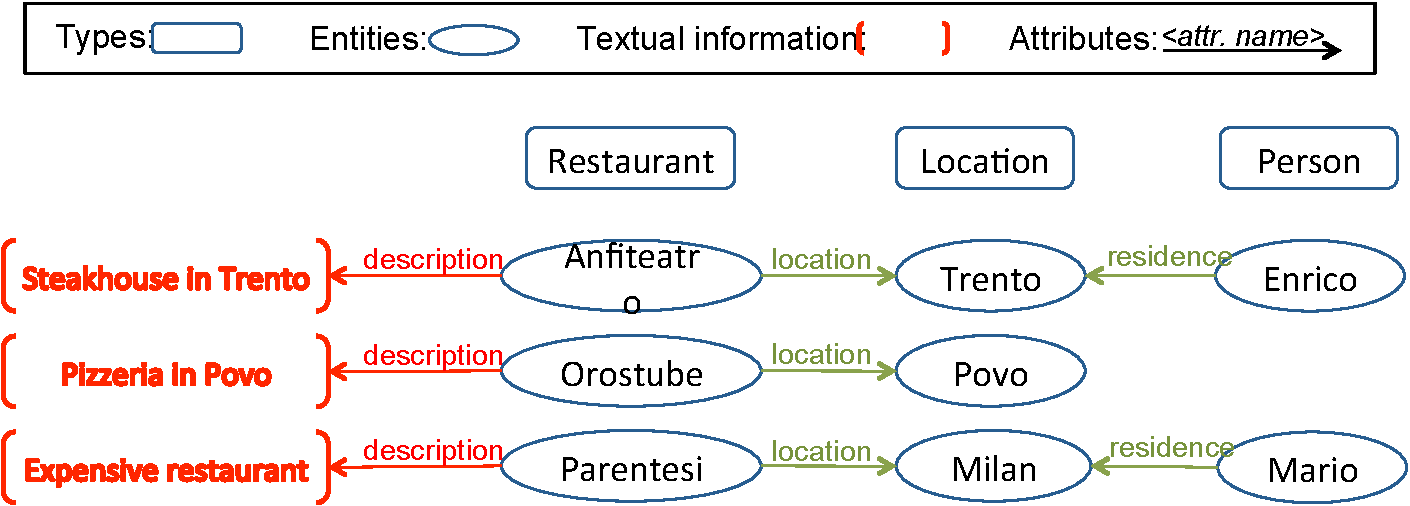
\includegraphics[width=0.90\textwidth]{figures/searchExample}
\caption{Example of simple entity repository}
\label{fig:search_example}
\end{figure}

The example entity repository has 3 entity types: \emph{Location}, \emph{Restaurant}, and \emph{Person}. Each entity type is instantiated by several entities. For instance, \emph{Trento}, \emph{Povo} and \emph{Milan} are names of entites of type \emph{Location}, \emph{Anfiteatro} is the name of a \emph{Restaurant} entity and \emph{Enrico} is the name of a \emph{Person} entity. Entities have different attributes, for instance, \emph{description} attribute of \emph{Location} entity contains textual information; while location attributes connect person and restaurant with locations correspondingly.

\paragraph{FROM clause.}
The simplest EQL query should contain at least the keyword \emph{from}, a type of entity, and an identifier for the resulting entities. For instance, in order to find all the restaurants stored in the entity repository, the query ``\texttt{FROM restaurant r}'' can be used.
%\begin{center}
%\begin{tabular}{l}
%\texttt{FROM restaurant r} \\
%\end{tabular}
%\end{center}
Note that there is no need to know the exact name of the entity type, concept search approach can also be used for matching entity types. For instance, in the case when there is a synonymy relationship between concepts \emph{restaurant} and \emph{bar} in the underlying knowledge base, the search to find all the restaurants can also be performed by using the query ``\texttt{FROM bar r}''.
%\begin{center}
%\begin{tabular}{l}
%\texttt{FROM bar r} \\
%\end{tabular}
%\end{center}

Another use of concept search query in \emph{from} clause can be to select a subset of all the entities for a given entity type. For instance, the following query finds only those restaurants that describe steakhouses:
\begin{center}
\begin{tabular}{l}
\texttt{FROM restaurant[description:steakhouse] r} \\
\end{tabular}
\end{center}
The query requires that descriptions of found restaurant entities contain complex concepts which are more specific than complex concept for `steakhouse', e.g. `steakhouse in Trento'.

\paragraph{SELECT clause.} 
The following query can be used to find descriptions and locations of all the restaurants. Which means to select attributes which are equivalent ore more specific than `description' and `location' of restaurant entities:
\begin{center}
\begin{tabular}{l}
\texttt{SELECT \textbf{restaurant1.description, restaurant1.location}} \\
\texttt{FROM restaurant \textbf{restaurant1}} \\
\end{tabular}
\end{center}
Note that also here there is no need to know the exact names for entity attributes. Equivalent or more general concepts can also be used. Moreover,
%For instance, we can search for related places with the query:
%\begin{center}
%\begin{tabular}{l}
%\texttt{SELECT restaurant1.description, \textbf{restaurant1.place}} \\
%\texttt{FROM restaurant restaurant1} \\
%\end{tabular}
%\end{center}
%Select 
the clause can also be used in combination with the selection of a subset of entities from a given type. For instance, find descriptions and related locations for all the steakhouses, i.e., select attributes which are equivalent ore more specific than `description' and `location' of restaurant entities with description containing complex concept (or concepts which are equivalent ore more specific than complex concept) `steakhouse':
\begin{center}
\begin{tabular}{l}
\texttt{SELECT restaurant1.description, \textbf{restaurant1.place}} \\ 
\texttt{FROM restaurant[\textbf{description:steakhouse}] restaurant1} \\
\end{tabular}
\end{center}

\paragraph{JOIN.}
Join on entities is probably the most important feature of EQL. For intance, the descriptions and location names for all the restaurants can be found with the following query:
\begin{center}
\begin{tabular}{l}
\texttt{SELECT restaurant1.description, location1.name} \\
\texttt{FROM \textbf{restaurant restaurant1 JOIN restaurant1.location location1}}
\end{tabular}
\end{center}
Note that an arbitrary number of joins is allowed with the following pattern:
\begin{center}
\begin{tabular}{l}
\texttt{... entity1 JOIN entity1.relationalAttribute entity2 ...}\\
\end{tabular}
\end{center}


\paragraph{GROUP BY, WHERE, and ORDER BY} clauses from HQL are supported also in EQL. Among them, the ORDER BY clause is of key importance because is the one that is used to implement the ranking of search results. For instance, to find the number of restaurants for each location and orders the results by location names (i.e., alphabetical order), we can use the query:
\begin{center}
\begin{tabular}{l}
\texttt{SELECT l.name, count(r)} \\
\texttt{FROM restaurant r join r.location l} \\
\texttt{GROUP BY l.name} \\
\texttt{ORDER BY l.name} \\
\end{tabular}
\end{center}
On the other hand, to order results by the number of restaurants on each location (i.e., numerical order), the following query can be used:
\begin{center}
\begin{tabular}{l}
\texttt{SELECT l.name, count(r)} \\
\texttt{FROM restaurant r join r.location l} \\
\texttt{GROUP BY l.name} \\
\texttt{ORDER BY count(r)} \\
\end{tabular}
\end{center}


\subsection{Limitations and Additional Notes}
It is also important to mention the \emph{current limitations}, which include:
\begin{enumerate}
\item \textbf{Joins:} Only inner join is supported, i.e., the keyword \emph{join} is used for specifying inner join.
\item \textbf{Nulls:} If an attribute name is selected, then only NOT NULL attribute values will be returned.

\begin{tabular}{ll}
\texttt{SELECT cat FROM Cat cat} & [all cats will be found] \\
\texttt{SELECT cat, cat.name FROM Cat cat} & [cats without names will be skipped] \\
\end{tabular}
\item \textbf{Aggregates:} Only simple aggregate functions on attributes are supported, e.g. count(cat).
\item \textbf{Dots:} As in HQL, dot-notation is used for accessing entity attributes. There are limitations on how dots are used. The first (and only the first) dot defines an attribute (e.g. cat.name). The second dot can be used only for accessing the meta-data (e.g. cat.name.metadata). Note, that it is not really a limitation because all the queries with two or more dots can be rewritten by using explicit joins, as it is shown below:

\begin{tabular}{p{0.45\textwidth}p{0.45\textwidth}}
\texttt{SELECT cat.mate.name} & [not supported] \\
\texttt{FROM Cat cat} & \\
 & \\
\texttt{SELECT mate.name}  & [equivalent query with explicit join] \\
\texttt{FROM Cat cat} & \\
\texttt{JOIN cat.mate mate} & \\
\end{tabular}
\end{enumerate}


The following are some \emph{additional notes} that are also important to take into account when interacting with the PM through EQL queries:
\begin{itemize}
\item If no attribute is specified in select or where clause, the entity id is used as a default attribute. For instance, 
``\texttt{SELECT cat FROM Cat cat}'' internally, will be translated to ``\texttt{SELECT cat.id FROM Cat cat}''

\item Specifying an alias (e.g. cat) is required. For instance, ``\texttt{FROM Cat cat}''

\item If concepts with multi-words are used for defining types or attributes, spaces between words should be replaced with underscore `\_'. For instance, ``\texttt{SELECT cat.first\_name FROM Cat cat}''.

\item Underscore `\_' can also be used for specifying correct concepts which should be used for attribute names and types. For instance, ``\texttt{SELECT cat.name\_123 FROM Cat\_321 cat}''.
\end{itemize}



%\subsubsection{Main Endpoints Documentation}
%\todo{The specification of the search APIs with an example will be added here for the final version of this document.}
%
%\begin{tabular}{llp{4cm}p{5cm}}
%\toprule
%Method & Api & Description & Example \\
%\midrule
%GET & /peers/search & Returns a set of profile of the peers that match with the characteristics specified in the input query & \\
%\bottomrule
%\end{tabular}













\newpage
\section{Peer Manager web API} \label{sec:pm-web-api-detail}
The following section specifies examples of the calls that the Proof of Concept version of the  Peer Manager accepts and the replies (example+format) that it produces. These are largely similar to what was reported last year (with minor usage-motivate changes), the bulk of the changes of this year implementation is reflected in the introduction of the PM abstraction API detailed in Appendix~\ref{sec:pm-abs-api-detail}.

\begin{figure*}[htb!]
\centering
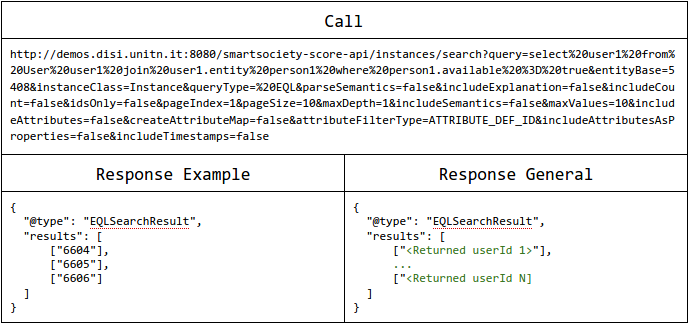
\includegraphics[width=1\linewidth]{figures/Peer-search.png}
\caption{Call and response for searching all available peers for a generic task. This call is used by WP6 (Orchestration) to obtain a list of users (that represent peers) that matches their set requirement.}
\label{fig:Peer-search}
\end{figure*}

\begin{figure*}[htb!]
\centering
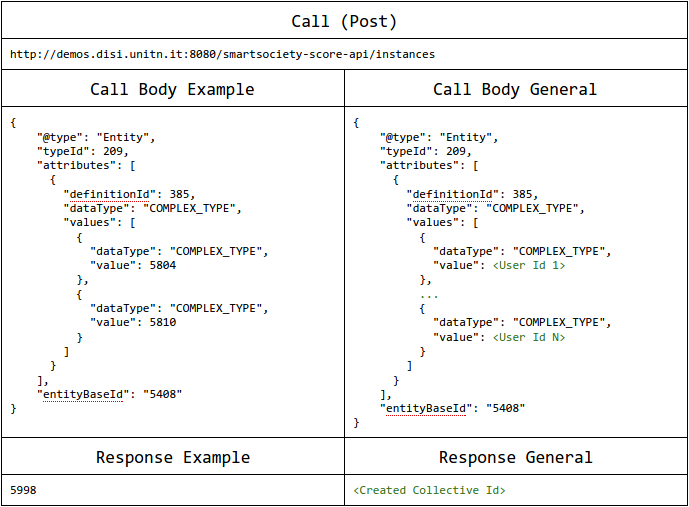
\includegraphics[width=1\linewidth]{figures/Collective-create.png}
\caption{Call and response for creating a new collective from a set of passed users. This call is used by the WP8 developed client to convert the list of users given by WP6 into a single Collective.}
\label{fig:Collective-create}
\end{figure*}

\begin{figure*}[htb!]
\centering
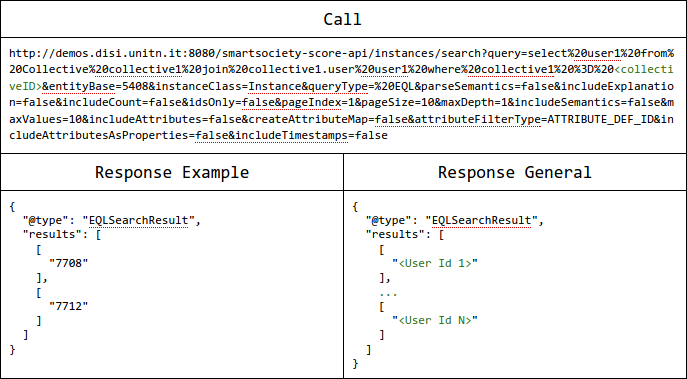
\includegraphics[width=1\linewidth]{figures/Collective-read.png}
\caption{Call and response for reading all the users from a given collective. WP7 (Middleware) uses this call to get the individual Users from a Collective with the intention of later contacting them.}
\label{fig:Collective-read}
\end{figure*}

\begin{figure*}[htb!]
\centering
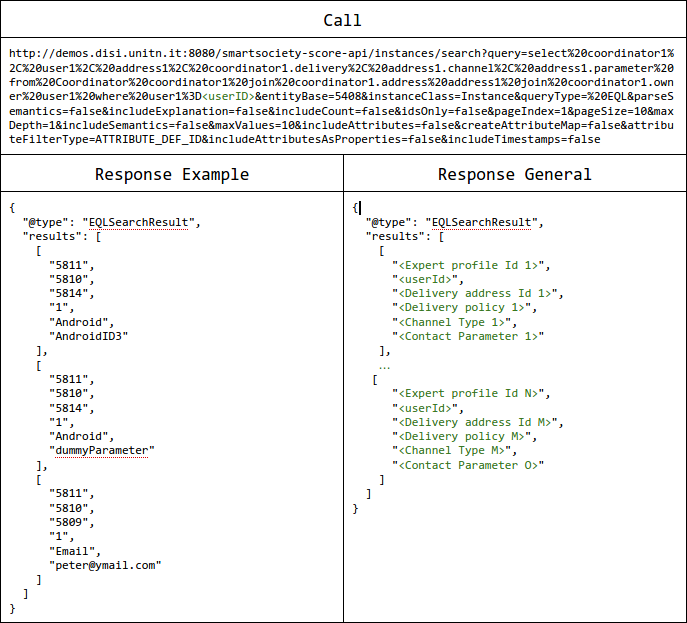
\includegraphics[width=1\linewidth]{figures/Peer-read.png}
\caption{Call and response for reading the contact information of a given peer. WP7 uses this call to get the specific contact preferences of a user in order to follow them when contacting that user.}
\label{fig:Peer-read}
\end{figure*}


\end{document}
